%
% grundaufgaben.tex
%
% (c) 2024 Prof Dr Andreas Müller
%
\begin{figure}
\centering
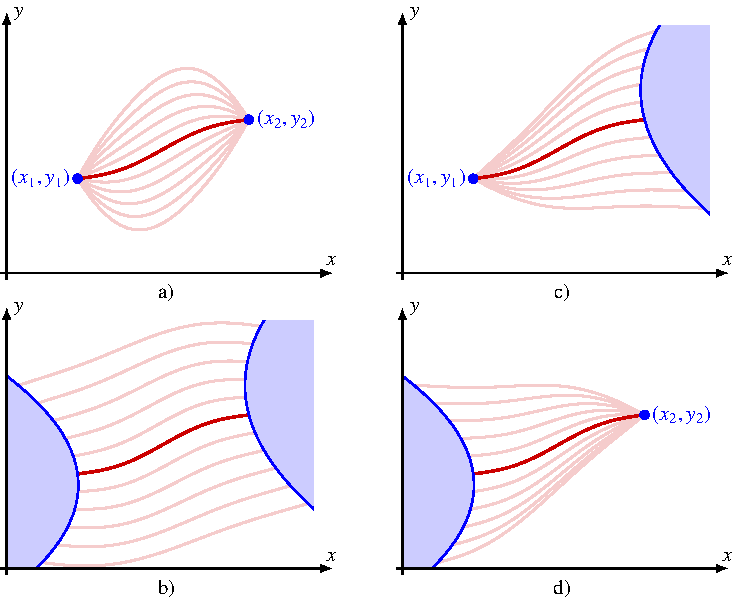
\includegraphics{chapters/020-variation/images/grundaufgaben.pdf}
\caption{Grundaufgaben der Variationsrechnung für eine Funktion $y(x)$.
a) Anfangspunkt-Endpunkt-Problem,
\index{Anfangspunkt-Endpunkt-Problem}%
b) Anfangskurve-Endkurve-Problem,
\index{Anfangskurve-Endkurve-Problem}%
c) Anfangspunkt-Endkurve-Problem,
\index{Anfangspunkt-Endkurve-Problem}%
d) Anfangspunkt-Endkurve-Problem
\index{Anfangspunkt-Endkurve-Problem}%
\label{buch:variation:problem:fig:grundaufgaben}}
\end{figure}
